\documentclass[../main.tex]{subfiles}

\begin{document}


\label{cha:cha_P_14} 
\chapter{General Linear Least-Squares and Nonlinear Regression}
\textbf{CHAPTER OBJECTIVES}

\noindent The primary objective of this chapter is to introduce you to how least-squares
regression can be used to fit a straight line to measured data. Specific objectives and
topics covered are

\begin{itemize}
	\item Familiarizing yourself with some basic descriptive statistics and the normal
	distribution.
	\item	 Knowing how to compute the slope and intercept of a best-fit straight line with
	linear regression.
	\item	 Knowing how to generate random numbers with MATLAB and how they can be
	employed for Monte Carlo simulations.
	\item	 Knowing how to compute and understand the meaning of the coefficient of
	determination and the standard error of the estimate.
	\item	 Understanding how to use transformations to linearize nonlinear equations so that
	they can be fit with linear regression.
	\item	 Knowing how to implement linear regression with MATLAB.
\end{itemize}

\noindent\textbf{YOU'VE GOT A PROBLEM}

\noindent In Chap. 1, we noted that a free-falling object such as a bungee jumper is subject to the upward force of air resistance. As a first approximation, we assumed that this force was proportional to the square of velocity as in

\begin{equation}
	\tag{14.1}
	F_U = c_d v^2
\end{equation}

\noindent where $F_U$ = the upward force of air resistance [N = kg m/s$^2$], $c_d$ = a drag coefficient
(kg/m), and $v$ = velocity [m/s].

Expressions such as Eq. (14.1) come from the field of fluid mechanics. Although such
relationships derive in part from theory, experiments play a critical role in their formulation. One such experiment is depicted in Fig. 14.1. An individual is suspended in a wind tunnel (any volunteers?) and the force measured for various levels of wind velocity. The
result might be as listed in Table 14.1.

\begin{figure}[H]
	\centering
	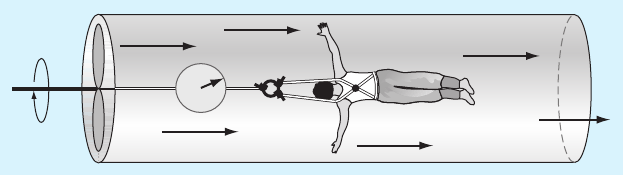
\includegraphics[width=0.5\linewidth]{fig_14_1}
	\caption{\textsf{Wind tunnel experiment to measure how the force of air resistance depends on velocity.}}
	\label{fig:fig_14_1}
\end{figure}

\begin{figure}[H]
	\centering
	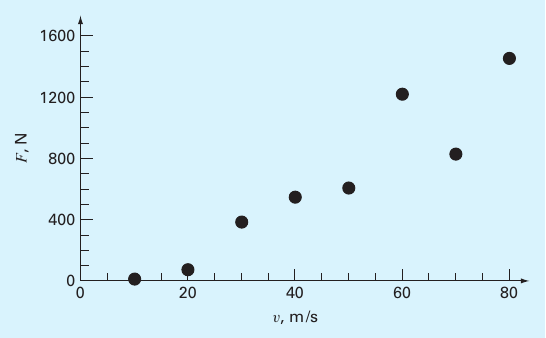
\includegraphics[width=0.5\linewidth]{fig_14_2}
	\caption{\textsf{Plot of force versus wind velocity for an object suspended in a wind tunnel.}}
	\label{fig:fig_14_2}
\end{figure}

\noindent \textbf{TABLE 14.1} Experimental data for force (N) and velocity (m/s) from a wind tunnel
experiment.

\begin{tabular}{l c c c ccccc}
	\textbf{$v$, m/s} & 10 & 20 & 30 & 40 & 50 & 60 & 70 & 80 \\
	\textbf{F, N} & 25 & 70 & 380 & 550 & 610 & 1220 & 830 & 1450
\end{tabular}

The relationship can be visualized by plotting force versus velocity. As in Fig. 14.2,
several features of the relationship bear mention. First, the points indicate that the force
increases as velocity increases. Second, the points do not increase smoothly, but exhibit
rather significant scatter, particularly at the higher velocities. Finally, although it may not
be obvious, the relationship between force and velocity may not be linear. This conclusion
becomes more apparent if we assume that force is zero for zero velocity.

In Chaps. 14 and 15, we will explore how to fit a ``best'' line or curve to such data. In
so doing, we will illustrate how relationships like Eq. (14.1) arise from experimental data.


\label{cha:cha_P_14_1}
\section{STATISTICS REVIEW}

\noindent Before describing least-squares regression, we will first review some basic concepts
from the field of statistics. These include the mean, standard deviation, residual sum of
the squares, and the normal distribution. In addition, we describe how simple descriptive
statistics and distributions can be generated in MATLAB. If you are familiar with these
subjects, feel free to skip the following pages and proceed directly to Section 14.2. If you
are unfamiliar with these concepts or are in need of a review, the following material is
designed as a brief introduction.

\label{cha:cha_P_14_1_1}
\subsection{Descriptive Statistics}

\noindent Suppose that in the course of an engineering study, several measurements were made of a
particular quantity. For example, Table 14.2 contains 24 readings of the coefficient of thermal expansion of a structural steel. Taken at face value, the data provide a limited amount
of information-that is, that the values range from a minimum of 6.395 to a maximum of
6.775. Additional insight can be gained by summarizing the data in one or more well-chosen statistics that convey as much information as possible about specific characteristics of
the data set. These descriptive statistics are most often selected to represent (1) the location
of the center of the distribution of the data and (2) the degree of spread of the data set.

\noindent \textbf{Measure of Location.} \quad The most common measure of central tendency is the arithmetic
mean. The arithmetic mean ($\bar{y}$) of a sample is defined as the sum of the individual data
points ($y_i$) divided by the number of points ($n$), or

\begin{equation}
	\tag{14.2}
	\bar{y} = \frac{\sum y_i}{n}
\end{equation}

where the summation (and all the succeeding summations in this section) is from $i$ = 1
through $n$.

There are several alternatives to the arithmetic mean. The \textit{median} is the midpoint of a
group of data. It is calculated by first putting the data in ascending order. If the number of
measurements is odd, the median is the middle value. If the number is even, it is the arithmetic mean of the two middle values. The median is sometimes called the \textit{50th percentile}.

The mode is the value that occurs most frequently. The concept usually has direct utility only when dealing with discrete or coarsely rounded data. For continuous variables such
as the data in Table 14.2, the concept is not very practical. For example, there are actually four modes for these data: 6.555, 6.625, 6.655, and 6.715, which all occur twice. If the numbers had not been rounded to 3 decimal digits, it would be unlikely that any of the values
would even have repeated twice. However, if continuous data are grouped into equispaced
intervals, it can be an informative statistic. We will return to the mode when we describe histograms later in this section.

\noindent \textbf{TABLE 14.2}	 \quad Measurements of the coefficient of thermal expansion of structural steel.

\begin{tabular}{ccccccccc}
	6.495 & 6.595 & 6.615 & 6.635 & 6.485 & 6.555 \\
	6.665 & 6.505 & 6.435 & 6.625 & 6.715 & 6.655 \\
	6.755 & 6.625 & 6.715 & 6.575 & 6.655 & 6.605 \\
	6.565 & 6.515 & 6.555 & 6.395 & 6.775 & 6.685
\end{tabular}

\noindent \textbf{Measures of Spread. } \quad  The simplest measure of spread is the \textit{range}, the difference between the largest and the smallest value. Although it is certainly easy to determine, it is not
considered a very reliable measure because it is highly sensitive to the sample size and is
very sensitive to extreme values.

The most common measure of spread for a sample is the \textit{standard deviation} ($s_ y$) about
the mean:

\begin{equation}
	\tag{14.3}
	s_y = \sqrt{\frac{S_t}{n-1}}
\end{equation}

\noindent where $S_t$ is the total sum of the squares of the residuals between the data points and the
mean, or

\begin{equation}
	\tag{14.4}
	S_t = \sum (y_i - \bar{y})^2
\end{equation}

\noindent Thus, if the individual measurements are spread out widely around the mean, $S_t$ (and, consequently, $s_y$) will be large. If they are grouped tightly, the standard deviation will be small.
The spread can also be represented by the square of the standard deviation, which is called
the \textit{variance}:

\begin{equation}
	\tag{14.5}
	s^2_y = \frac{\sum (y_i - \bar{y})^2}{n-1}
\end{equation}

Note that the denominator in both Eqs. (14.3) and (14.5) is $n - 1$. The quantity $n - 1$
is referred to as the \textit{degrees of freedom}. Hence $S_t$ and $s_y$ are said to be based on $n - 1$ degrees of freedom. This nomenclature derives from the fact that the sum of the quantities
upon which $S_t$ is based (i.e., $\bar{y} - y_1 , \bar{y} - y_2 , \dots , \bar{y} - y_n$) is zero. Consequently, if $\bar{y}$ is
known and $n - 1$ of the values are specified, the remaining value is fixed. Thus, only $n - 1$
of the values are said to be freely determined. Another justification for dividing by $n - 1$ is
the fact that there is no such thing as the spread of a single data point. For the case where
$n = 1$, Eqs. (14.3) and (14.5) yield a meaningless result of infinity.

We should note that an alternative, more convenient formula is available to compute
the variance:

\begin{equation}
	\tag{14.6}
	s^2_y = \frac{\sum y_i^2 -(\sum y_i)^2 / n}{n-1}
\end{equation}

\noindent This version does not require precomputation of $\bar{y}$ and yields an identical result as Eq. (14.5).

A final statistic that has utility in quantifying the spread of data is the coefficient of
variation (c.v.). This statistic is the ratio of the standard deviation to the mean. As such, it
provides a normalized measure of the spread. It is often multiplied by 100 so that it can be
expressed in the form of a percent:

\begin{equation}
	\tag{14.7}
	\text{c.v.} = \frac{s_y}{\bar{y}} \times 100\%
\end{equation}

\begin{example} Simple Statistics of a Sample
	
	\noindent \textbf{Problem Statement.} \quad Compute the mean, median, variance, standard deviation, and coefficient of variation for the data in Table 14.2.

	\noindent \textbf{Solution.} \quad   The data can be assembled in tabular form and the necessary sums computed
	as in Table 14.3.

	The mean can be computed as [Eq. (14.2)],

	$$
		\bar{y} = \frac{158.4}{24} = 6.6
	$$

	\noindent Because there are an even number of values, the median is computed as the arithmetic
	mean of the middle two values: (6.605 + 6.615)/2 = 6.61.

	As in Table 14.3, the sum of the squares of the residuals is 0.217000, which can be
used to compute the standard deviation [Eq. (14.3)]:

	$$
		s_y = \sqrt{\frac{0.217000}{24 - 1}}  = 0.097133
	$$

	\noindent \textbf{TABLE 14.3} \quad Data and summations for computing simple descriptive statistics for the
	coefficients of thermal expansion from Table 14.2.

	\begin{tabular}{cccc}
		$i$ & $y_i$ & $(y_i - \bar{y})^2$ & $y_i^2$\\
		\hline
		1 & 6.395 & 0.04203 & 40.896 \\
		2 & 6.435 & 0.02723 & 41.409 \\
		3 & 6.485 & 0.01323 & 42.055 \\
		4 & 6.495 & 0.01103 & 42.185 \\
		5 & 6.505 & 0.00903 & 42.315 \\
		6 & 6.515 & 0.00723 & 42.445 \\
		7 & 6.555 & 0.00203 & 42.968 \\
		8 & 6.555 & 0.00203 & 42.968 \\
		9 & 6.565 & 0.00123 & 43.099 \\ 
		10 & 6.575 & 0.00063 & 43.231 \\
		11 & 6.595 & 0.00003 & 43.494 \\
		12 & 6.605 & 0.00002 & 43.626 \\ 
		13 & 6.615 & 0.00022 & 43.758 \\
		14 & 6.625 & 0.00062 & 43.891 \\
		15 & 6.625 & 0.00062 & 43.891 \\ 
		16 & 6.635 & 0.00122 & 44.023 \\
		17 & 6.655 & 0.00302 & 44.289 \\
		18 & 6.655 & 0.00302 & 44.289 \\ 
		19 & 6.665 & 0.00422 & 44.422 \\
		20 & 6.685 & 0.00722 & 44.689 \\
		21 & 6.715 & 0.01322 & 45.091 \\ 
		22 & 6.715 & 0.01322 & 45.091 \\
		23 & 6.755 & 0.02402 & 45.630 \\
		24 & 6.775 & 0.03062 & 45.901 \\ 
		$\sum$ &158.400 & 0.21700 & 1045.657
	\end{tabular}

	\noindent the variance [Eq. (14.5)]:

	$$
	s^2_y = (0.097133)^2 = 0.009435
	$$

	\noindent and the coefficient of variation [Eq. (14.7)]:

	$$
		\text{c.v.} = \frac{0.097133}{6.6 } \times 100\% = 1.47\%
	$$

	\noindent The validity of Eq. (14.6) can also be verified by computing

	$$
		s^2_y = \frac{1045.657 - (158.400)^2 /24}{24 - 1} = 0.009435
	$$

\end{example}

\label{cha:cha_P_14_1_2}
\subsection{The Normal Distribution}

\noindent Another characteristic that bears on the present discussion is the data distribution-that is,
the shape with which the data are spread around the mean. A histogram provides a simple
visual representation of the distribution. A \textit{histogram} is constructed by sorting the measurements into intervals, or \textit{bins}. The units of measurement are plotted on the abscissa and
the frequency of occurrence of each interval is plotted on the ordinate.

As an example, a histogram can be created for the data from Table 14.2. The result
(Fig. 14.3) suggests that most of the data are grouped close to the mean value of 6.6.
Notice also, that now that we have grouped the data, we can see that the bin with the most
values is from 6.6 to 6.64. Although we could say that the mode is the midpoint of this bin,
6.62, it is more common to report the most frequent range as the \textit{modal class interval}.

If we have a very large set of data, the histogram often can be approximated by a
smooth curve. The symmetric, bell-shaped curve superimposed on Fig. 14.3 is one such
characteristic shape-the \textit{normal distribution}. Given enough additional measurements, the
histogram for this particular case could eventually approach the normal distribution.


\begin{figure}[H]
	\centering
	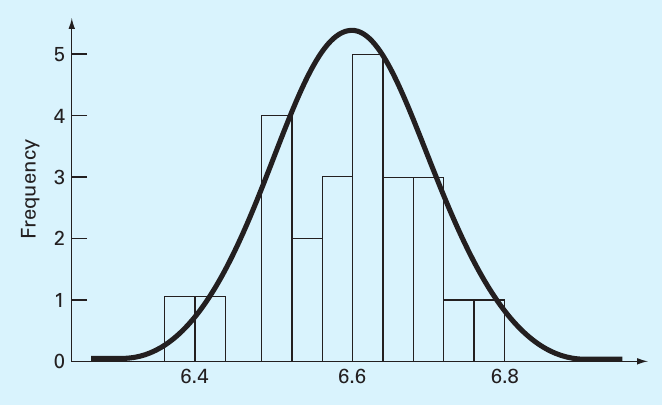
\includegraphics[width=0.5\linewidth]{fig_14_3}
	\caption{\textsf{A histogram used to depict the distribution of data. As the number of data points increases, the
	histogram often approaches the smooth, bell-shaped curve called the normal distribution.}}
	\label{fig:fig_14_3}
\end{figure}

The concepts of the mean, standard deviation, residual sum of the squares, and normal distribution all have great relevance to engineering and science. A very simple exam-
ple is their use to quantify the confidence that can be ascribed to a particular measurement.
If a quantity is normally distributed, the range defined by $\bar{y} - s_y$ to $\bar{y} + s_y$ will encompass
approximately 68\% of the total measurements. Similarly, the range defined by $\bar{y} -  2s_y$ to
$\bar{y} + 2s_ y$ will encompass approximately 95\%.

For example, for the data in Table 14.2, we calculated in Example 14.1 that $\bar{y} = 6.6$
and $s_y = 0.097133$. Based on our analysis, we can tentatively make the statement that
approximately 95\% of the readings should fall between 6.405734 and 6.794266. Because it
is so far outside these bounds, if someone told us that they had measured a value of 7.35, we
would suspect that the measurement might be erroneous.

\label{cha:cha_P_14_1_3}
\subsection{Descriptive Statistics in MATLAB}

\noindent Standard MATLAB has several functions to compute descriptive statistics. For example,
the arithmetic mean is computed as \texttt{mean(x)}. If \texttt{x} is a vector, the function returns the mean
of the vector's values. If it is a matrix, it returns a row vector containing the arithmetic
mean of each column of \texttt{x}. The following is the result of using mean and the other statistical functions to analyze a column vector s that holds the data from Table 14.2:

\begin{lstlisting}[numbers=none]
	>> format short g
	>> mean(s),median(s),mode(s)
	ans =
		6.6
	ans =
		6.61
	ans =
		6.555
	>> min(s),max(s)
	ans =
		6.395
	ans =
		6.775
	>> range=max(s)-min(s)
	range =
		0.38
	>> var(s),std(s)
	ans =
		0.0094348
	ans =
		0.097133
\end{lstlisting}

\noindent These results are consistent with those obtained previously in Example 14.1. Note that
although there are four values that occur twice, the mode function only returns the first of
the values: 6.555.

\begin{figure}[H]
	\centering
	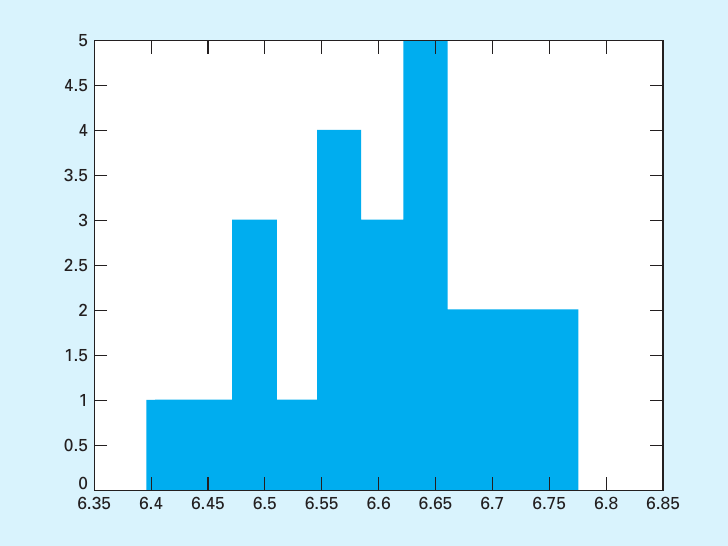
\includegraphics[width=0.5\linewidth]{fig_14_4}
	\caption{\textsf{Histogram generated with the MATLAB \texttt{hist} function.}}
	\label{fig:fig_14_4}
\end{figure}

MATLAB can also be used to generate a histogram based on the \texttt{hist}  function. The
hist function has the syntax

\begin{lstlisting}[numbers=none]
	[n, x] = hist(y, x)
\end{lstlisting}

\noindent where \texttt{n} = the number of elements in each bin, \texttt{x} = a vector specifying the midpoint of
each bin, and \texttt{y} is the vector being analyzed. For the data from Table 14.2, the result is

\begin{lstlisting}[numbers=none]
	>> [n,x] =hist(s)
	n =	
		1	1	3	1	4	3	5	2	2	2
	x =
		6.414 6.452 6.49 6.528 6.566 6.604 6.642 6.68 6.718 6.756
\end{lstlisting}

The resulting histogram depicted in Fig. 14.4 is similar to the one we generated by hand in
Fig. 14.3. Note that all the arguments and outputs with the exception of \texttt{y} are optional. For
example, \texttt{hist(y)} without output arguments just produces a histogram bar plot with
10 bins determined automatically based on the range of values in \texttt{y}.

\label{cha:cha_P_14_2}
\section{RANDOM NUMBERS AND SIMULATION}
\noindent In this section, we will describe two MATLAB functions that can be used to produce a
sequence of random numbers. The first (\texttt{rand}) generates numbers that are uniformly
distributed, and the second (\texttt{randn}) generates numbers that have a normal distribution.

\label{cha:cha_P_14_2_1}
\subsection{MATLAB Function: \texttt{rand}}

\noindent This function generates a sequence of numbers that are uniformly distributed between 0
and 1. A simple representation of its syntax is

\begin{lstlisting}[numbers=none]
	r = rand(m, n)
\end{lstlisting}

\noindent where \texttt{r} = an \texttt{m}-by-\texttt{n} matrix of random numbers. The following formula can then be used
to generate a uniform distribution on another interval:

\begin{lstlisting}[numbers=none]
	runiform = low + (up - low) * rand(m, n)
\end{lstlisting}

\noindent where \texttt{low} = the lower bound and \texttt{up} = the upper bound.

\begin{example} Generating Uniform Random Values of Drag

	\noindent \textbf{Problem Statement. } \quad  If the initial velocity is zero, the downward velocity of the free-falling
	bungee jumper can be predicted with the following analytical solution (Eq. 1.9):

	$$
		v= \sqrt{\frac{gm}{c_d} } \tanh \left(\sqrt{\frac{gc_d}{m} t}\right)
	$$

	\noindent Suppose that $g = 9.81$ m/s$^2$ , and $m$ = 68.1 kg, but $c_d$ is not known precisely. For example,
	you might know that it varies uniformly between 0.225 and 0.275 (i.e., $\pm 10\%$ around a
	mean value of 0.25 kg/m). Use the \texttt{rand} function to generate 1000 random uniformly
	distributed values of $c_d$ and then employ these values along with the analytical solution to
	compute the resulting distribution of velocities at $t$ = 4 s.

	\noindent \textbf{Solution. } \quad  Before generating the random numbers, we can first compute the mean velocity:

	$$
		v_{\text{mean}} = \sqrt{\frac{9.81(68.1)}{0.25}} \tanh \left(\sqrt{\frac{9.81(0.25)}{68.1}} 4 \right) = 33.1118 \frac{m}{s}
	$$

	\noindent We can also generate the range:

	$$
		v_{\text{low}} = \sqrt{\frac{9.81(68.1)}{0.275}} \tanh \left(\sqrt{\frac{9.81(0.275)}{68.1}} 4 \right) = 32.6223 \frac{m}{s}
	$$

	$$
		v_{\text{high}} = \sqrt{\frac{9.81(68.1)}{0.225}} \tanh \left(\sqrt{\frac{9.81(0.225)}{68.1}} 4 \right) = 33.6198 \frac{m}{s}
	$$

	\noindent Thus, we can see that the velocity varies by

	$$
		\Delta v = \frac{33.6198 - 32.6223}{2(33.1118)} \times 100 \% = 1.5063\%
	$$

	\noindent The following script generates the random values for $c_d$ , along with their mean, standard
	deviation, percent variation, and a histogram:

	\begin{lstlisting}[numbers=none]
		clc,format short g
		n=1000;t=4;m=68.1;g=9.81;
		cd=0.25;cdmin=cd-0.025,cdmax=cd+0.025
		r=rand(n,1);
		cdrand=cdmin+(cdmax-cdmin)*r;
		meancd=mean(cdrand),stdcd=std(cdrand)
		Deltacd=(max(cdrand)-min(cdrand))/meancd/2*100.
		subplot(2,1,1)
		hist(cdrand),title('(a) Distribution of drag')
		xlabel('cd (kg/m)')
	\end{lstlisting}

	\noindent The results are

	\begin{lstlisting}[numbers=none]
		meancd =
			0.25018
		stdcd =
			0.014528
		Deltacd =
			9.9762
	\end{lstlisting}

	\noindent These results, as well as the histogram (Fig. 14.5a) indicate that \texttt{rand} has yielded 1000
	uniformly distributed values with the desired mean value and range. The values can then be
	employed along with the analytical solution to compute the resulting distribution of velocities at $t$ = 4 s.

	\begin{figure}[H]
		\centering
		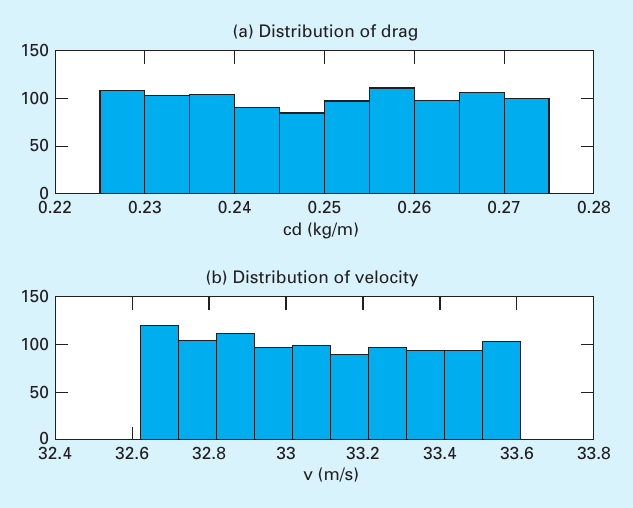
\includegraphics[width=0.5\linewidth]{fig_14_5}
		\caption{\textsf{Histograms of (a) uniformly distributed drag coefficients and (b) the resulting distribution of velocity.}}
		\label{fig:fig_14_5}
	\end{figure}

	\begin{lstlisting}[numbers=none]
		vrand=sqrt(g*m./cdrand).*tanh(sqrt(g*cdrand/m)*t);
		meanv=mean(vrand)
		Deltav=(max(vrand)-min(vrand))/meanv/2*100.
		subplot(2,1,2)
		hist(vrand),title('(b) Distribution of velocity')
		xlabel('v (m/s)')
	\end{lstlisting}

	\noindent The results are

	\begin{lstlisting}[numbers=none]
		meanv =
			33.1151
		Deltav =
			1.5048
	\end{lstlisting}

	\noindent These results, as well as the histogram (Fig. 14.5b), closely conform to our hand calculations.
\end{example}

The foregoing example is formally referred to as a \textit{Monte Carlo simulation}. The term,
which is a reference to Monaco's Monte Carlo casino, was first used by physicists working
on nuclear weapons projects in the 1940s. Although it yields intuitive results for this simple
example, there are instances where such computer simulations yield surprising outcomes
and provide insights that would otherwise be impossible to determine. The approach is feasible only because of the computer's ability to implement tedious, repetitive computations
in an efficient manner.

\label{cha:cha_P_14_2_2}
\subsection{MATLAB Function: \texttt{randn}}

\noindent This function generates a sequence of numbers that are normally distributed with a mean
of 0 and a standard deviation of 1. A simple representation of its syntax is

\begin{lstlisting}[numbers=none]
	r = randn(m, n)
\end{lstlisting}

\noindent where \texttt{r} = an \texttt{m}-by-\texttt{n} matrix of random numbers. The following formula can then be used
to generate a normal distribution with a different mean (\texttt{mn}) and standard deviation (s),

\begin{lstlisting}[numbers=none]
	rnormal = mn + s * randn(m, n)
\end{lstlisting}

\begin{example} Generating Normally-Distributed Random Values of Drag
	
	\noindent \textbf{Problem Statement. } \quad Analyze the same case as in Example 14.2, but rather than employing a uniform distribution, generate normally-distributed drag coefficients with a mean of
	0.25 and a standard deviation of 0.01443.

	\noindent \textbf{Solution. } \quad The following script generates the random values for $c_d$ , along with their mean,
	standard deviation, coefficient of variation (expressed as a \%), and a histogram:

	\begin{lstlisting}[numbers=none]
		clc,format short g
		n=1000;t=4;m=68.1;g=9.81;
		cd=0.25;
		stdev=0.01443;
		r=randn(n,1);
		cdrand=cd+stdev*r;
		meancd=mean(cdrand),stdevcd=std(cdrand)
		cvcd=stdevcd/meancd*100.
		subplot(2,1,1)
		hist(cdrand),title('(a) Distribution of drag')
		xlabel('cd (kg/m)')
	\end{lstlisting}

	\noindent  The results are

	\begin{lstlisting}[numbers=none]
		meancd =
			0.24988
		stdevcd =
			0.014465
		cvcd =
			5.7887
	\end{lstlisting}

	\noindent These results, as well as the histogram (Fig. 14.6a) indicate that randn has yielded 1000
	uniformly distributed values with the desired mean, standard deviation, and coefficient
	of variation. The values can then be employed along with the analytical solution to compute the resulting distribution of velocities at $t$ = 4 s.

	\begin{lstlisting}[numbers=none]
		vrand=sqrt(g*m./cdrand).*tanh(sqrt(g*cdrand/m)*t);
		meanv=mean(vrand),stdevv=std(vrand)
		cvv=stdevv/meanv*100.
		subplot(2,1,2)
		hist(vrand),title('(b) Distribution of velocity')
		xlabel('v (m/s)')
	\end{lstlisting}

	\noindent The results are

	\begin{lstlisting}[numbers=none]
		meanv =
			33.117
		stdevv =
			0.28839
		cvv =
			0.8708
	\end{lstlisting}

	\noindent These results, as well as the histogram (Fig. 14.6b), indicate that the velocities are also normally distributed with a mean that is close to the value that would be computed using the
	mean and the analytical solution. In addition, we compute the associated standard deviation
	which corresponds to a coefficient of variation of $\pm 0.8708\%$.

	\begin{figure}[H]
		\centering
		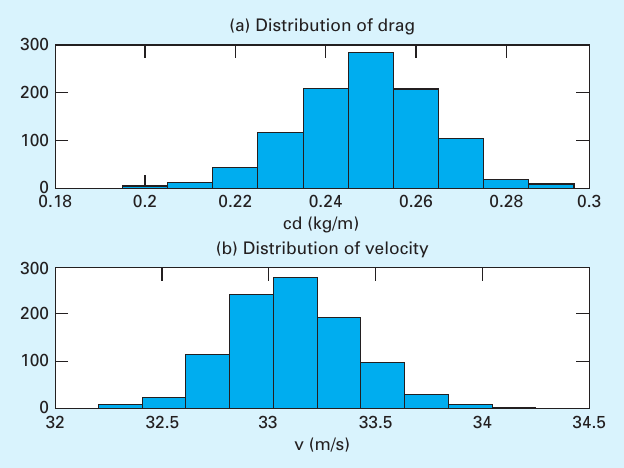
\includegraphics[width=0.5\linewidth]{fig_14_6}
		\caption{\textsf{Histograms of (a) normally-distributed drag coefficients and (b) the resulting distribution of velocity.}}
		\label{fig:fig_14_6}
	\end{figure}
\end{example}

Although simple, the foregoing examples illustrate how random numbers can be easily generated within MATLAB. We will explore additional applications in the end-of-chapter problems.

\label{cha:cha_P_14_3}
\section{LINEAR LEAST-SQUARES REGRESSION}

\noindent Where substantial error is associated with data, the best curve-fitting strategy is to derive
an approximating function that fits the shape or general trend of the data without necessarily matching the individual points. One approach to do this is to visually inspect the
plotted data and then sketch a ``best'' line through the points. Although such ``eyeball''
approaches have commonsense appeal and are valid for ``back-of-the-envelope'' calculations, they are deficient because they are arbitrary. That is, unless the points define a perfect
straight line (in which case, interpolation would be appropriate), different analysts would
draw different lines.

To remove this subjectivity, some criterion must be devised to establish a basis for the
fit. One way to do this is to derive a curve that minimizes the discrepancy between the data
points and the curve. To do this, we must first quantify the discrepancy. The simplest example is fitting a straight line to a set of paired observations: $(x_1 , y_1 ), (x_2 , y_2 ), \dots , (x_n , y_n )$.
The mathematical expression for the straight line is

\begin{equation}
	tag{14.8}
	y = a_0 + a_1 x +e
\end{equation}

where $a_0$ and $a_1$ are coefficients representing the intercept and the slope, respectively, and
e is the error, or \textit{residual}, between the model and the observations, which can be represented by rearranging Eq. (14.8) as

\begin{equation}
	\tag{14.9}
	e = y - a_0 - a_1 x
\end{equation}

\noindent Thus, the residual is the discrepancy between the true value of $y$ and the approximate value,
$a_0 + a_1 x$, predicted by the linear equation.

\label{cha:cha_P_14_3_1}
\subsection{Criteria for a ``Best'' Fit}

\noindent One strategy for fitting a ``best'' line through the data would be to minimize the sum of the
residual errors for all the available data, as in

\begin{equation}
	\tag{14.10}
	\sum_{i=1}^n e_i = \sum^n_{i=1} (y_i - a_0 - a_1 x_i)
\end{equation}

where $n$ = total number of points. However, this is an inadequate criterion, as illustrated by
Fig. 14.7a, which depicts the fit of a straight line to two points. Obviously, the best fit is the
line connecting the points. However, any straight line passing through the midpoint of the
connecting line (except a perfectly vertical line) results in a minimum value of Eq. (14.10)
equal to zero because positive and negative errors cancel.

One way to remove the effect of the signs might be to minimize the sum of the absolute values of the discrepancies, as in

\begin{equation}
	\tag{14.11}
	\sum_{i=1}^n \left| e_i \right| = \sum^n_{i=1} \left| y_i - a_0 - a_1 x_i \right|
\end{equation}

\noindent Figure 14.7b demonstrates why this criterion is also inadequate. For the four points shown,
any straight line falling within the dashed lines will minimize the sum of the absolute values of the residuals. Thus, this criterion also does not yield a unique best fit.

\begin{figure}[H]
	\centering
	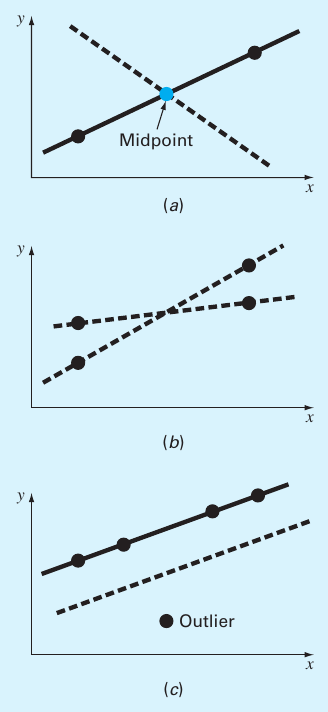
\includegraphics[width=0.5\linewidth]{fig_14_7} % ups
	\caption{\textsf{Examples of some criteria for ``best fit'' that are inadequate for regression: (a) minimizes the sum
	of the residuals, (b) minimizes the sum of the absolute values of the residuals, and (c) minimizes
	the maximum error of any individual point.}}
	\label{fig:fig_14_7}
\end{figure}

A third strategy for fitting a best line is the \textit{minimax} criterion. In this technique, the line
is chosen that minimizes the maximum distance that an individual point falls from the line.
As depicted in Fig. 14.7c, this strategy is ill-suited for regression because it gives undue
influence to an outlier-that is, a single point with a large error. It should be noted that
the minimax principle is sometimes well-suited for fitting a simple function to a complicated function (Carnahan, Luther, and Wilkes, 1969).

A strategy that overcomes the shortcomings of the aforementioned approaches is to
minimize the sum of the squares of the residuals:

\begin{equation}
	\tag{14.12}
	S_r = \sum_{i=1}^n e_i^2 = \sum^n_{i=1} (y_i - a_0 - a_1 x_i)^2
\end{equation}

\noindent This criterion, which is called \textit{least squares}, has a number of advantages, including that it
yields a unique line for a given set of data. Before discussing these properties, we will present a technique for determining the values of $a_0$ and $a_1$ that minimize Eq. (14.12).

\label{cha:cha_P_14_3_2}
\subsection{Least-Squares Fit of a Straight Line}

\noindent To determine values for $a_0$ and $a_1$ , Eq. (14.12) is differentiated with respect to each
unknown coefficient:

\begin{equation}
	\notag
	\frac{\partial S_r}{\partial a_0} = -2 \sum (y_i - a_0 - a_1 x_i)
\end{equation}

\begin{equation}
	\notag
	\frac{\partial S_r}{\partial a_1} = -2 \sum [(y_i - a_0 - a_1 x_i) x_i]
\end{equation}

\noindent Note that we have simplified the summation symbols; unless otherwise indicated, all summations are from $i = 1$ to $n$. Setting these derivatives equal to zero will result in a minimum
$S_r$. If this is done, the equations can be expressed as

\begin{equation}
	\notag
	0 = \sum y_i - \sum a_0 - \sum a_1 x_i
\end{equation}

\begin{equation}
	\notag
	0 = \sum x_i y_i - \sum a_0 x_i - \sum a_1 x_i^2
\end{equation}

\noindent Now, realizing that $\sum a_0 = na_0$, we can express the equations as a set of two simultaneous
linear equations with two unknowns ($a_0$ and $a_1$):

\begin{equation}
	\tag{14.13}
	n \quad a_0 + \left( \sum x_i \right) a_1 = \sum y_i
\end{equation}

\begin{equation}
	\tag{14.14}
	\left( \sum x_i \right) a_0 + \left( \sum x_i^2 \right) a_1 = \sum x_i y_i
\end{equation}

\noindent These are called the \textit{normal equations}. They can be solved simultaneously for

\begin{equation}
	\tag{14.15}
	a_1 = \frac{n \sum x_i y_i - \sum x_i \sum y_i}{n \sum x^2_i - \left( \sum x_i \right) ^ 2}
\end{equation}

\noindent This result can then be used in conjunction with Eq. (14.13) to solve for

\begin{equation}
	\tag{14.16}
	a_0 = \bar{y} - a_1 \bar{x}
\end{equation}

\noindent where $\bar{y}$ and $\bar{x}$ are the means of $y$ and $x$, respectively.

\begin{example} Linear Regression
	
	\noindent \textbf{Problem Statement. } \quad  Fit a straight line to the values in Table 14.1.

	\noindent \textbf{Solution. } \quad   In this application, force is the dependent variable ($y$) and velocity is the
	independent variable ($x$). The data can be set up in tabular form and the necessary sums
	computed as in Table 14.4.

	\noindent \textbf{TABLE 14.4} \quad Data and summations needed to compute the best-fit line for the data
	from Table 14.1.

	\begin{tabular}{lrrrr}
		$i$ & $x_i$ & $y_i$ & $x^2_i$ & $x_i y_i$ \\
		\hline
		1 & 10 & 25 & 100 & 250 \\
		2 & 20 & 70 & 400 & 1,400 \\
		3 & 30 & 380 & 900 & 11,400 \\
		4 & 40 & 550 & 1,600 & 22,000 \\
		5 & 50 & 610 & 2,500 & 30,500 \\
		6 & 60 & 1,220 & 3,600 & 73,200 \\
		7 & 70 & 830 & 4,900 & 58,100 \\
		8 & 80 & 1,450 & 6,400 & 116,000 \\
		$\sum$ &360 & 5,135 & 20,400 & 312,850
	\end{tabular}

	The means can be computed as

	$$
		\bar{x} = \frac{360}{8} = 45 \quad \bar{y} = \frac{5,135}{8 } = 641.875
	$$

	\noindent The slope and the intercept can then be calculated with Eqs. (14.15) and (14.16) as

	$$
		a_1 = \frac{8(312,850) - 360(5,135)}{8(20,400) - (360)^2} = 19.47024
	$$

	$$
		a_0 = 641.875 - 19.47024(45) = -234.2857
	$$

	\noindent Using force and velocity in place of y and x, the least-squares fit is

	$$
	F = -234.2857 + 19.47024v
	$$

	\noindent The line, along with the data, is shown in Fig. 14.8.

	\begin{figure}[H]
		\centering
		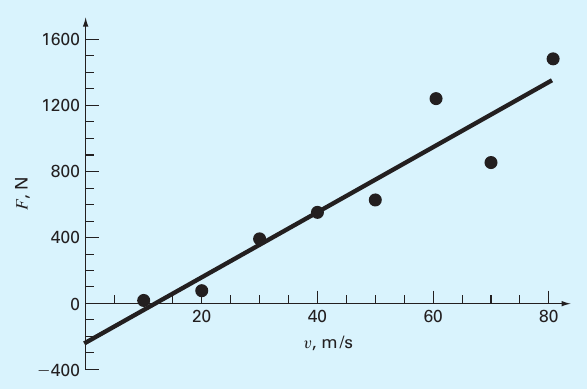
\includegraphics[width=0.5\linewidth]{fig_14_8}
		\caption{\textsf{Least-squares fit of a straight line to the data from Table 14.1}}
		\label{fig:fig_14_8}
	\end{figure}

	Notice that although the line fits the data well, the zero intercept means that the equation predicts physically unrealistic negative forces at low velocities. In Section 14.4, we
will show how transformations can be employed to derive an alternative best-fit line that is
more physically realistic.

\end{example}



\label{cha:cha_P_14_3_3}
\subsection{Quantification of Error of Linear Regression}

\noindent Any line other than the one computed in Example 14.4 results in a larger sum of the squares of the residuals. Thus, the line is unique and in terms of our chosen criterion is a ``best'' line through the points. A number of additional properties of this fit can be elucidated by examining more closely the way in which residuals were computed. Recall that the sum of the squares is defined as [Eq. (14.12)]

\begin{equation}
	\tag{14.17}
	S_r = \sum^n_{i=1} (y_i - a_0 - a_1 x_i)^2
\end{equation}

Notice the similarity between this equation and Eq. (14.4)

\begin{equation}
\tag{14.18}
S_t = \sum (y_i - \bar{y})^2
\end{equation}
In Eq. (14.18), the square of the residual represented the square of the discrepancy between the data and a single estimate of the measure of central tendency-the mean. In Eq. (14.17), the square of the residual represents the square of the vertical distance between the data and another measure of central tendency-the straight line (\ref{fig:fig_14_9}).

\begin{wrapfigure}{l}{0.25\textwidth}
    \centering
    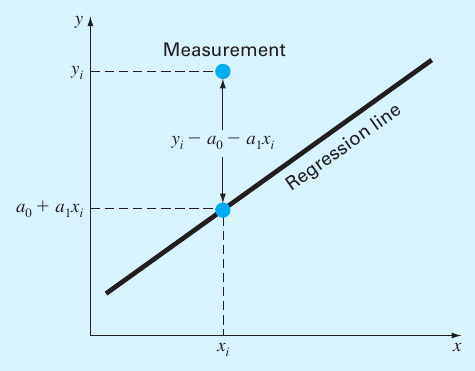
\includegraphics[width=0.25\textwidth]{fig_14_9}
   \caption{\textsf{The residual in linear regression represents the vertical distance between a data point and the straight line.}}
   \label{fig:fig_14_9}
\end{wrapfigure}

The analogy can be extended further for cases where (1) the spread of the points around the line is of similar magnitude along the entire range of the data and (2) the distribution of these points about the line is normal. It can be demonstrated that if these criteria are met, least-squares regression will provide the best (i.e., the most likely) estimates of $a_0$ and $a_1$ (Draper and Smith, 1981). This is called the maximum likelihood principle in statistics. In addition, if these criteria are met, a ``standard deviation'' for the regression line can be determined as [compare with Eq. (14.3)]

\begin{equation}
	\tag{14.19}
	s_{y/x} = \sqrt{\frac{S_r}{n-2}}
\end{equation}

\noindent where $s_{y/x}$ is called the \textit{standard error of the estimate}. The subscript notation ``$y/x$'' designates that the error is for a predicted value of $y$ corresponding to a particular value of $x$.
Also, notice that we now divide by $n - 2$ because two data-derived estimates - $a_0$ and $a_1$ - were used to compute $S_r$; thus, we have lost two degrees of freedom. As with our discussion of the standard deviation, another justification for dividing by $n - 2$ is that there is no such thing as the ``spread of data'' around a straight line connecting two points. Thus, for the case where $n = 2$, Eq. (14.19) yields a meaningless result of infinity.

Just as was the case with the standard deviation, the standard error of the estimate quantifies the spread of the data. However, $s_{y/x}$ quantifies the spread \textit{around the regression line} as shown in \ref{fig:fig_14_10b} in contrast to the standard deviation $s_y$ that quantified the \textit{spread around the mean} (\ref{fig:fig_14_10a}).

\begin{figure}[H]
	\centering
	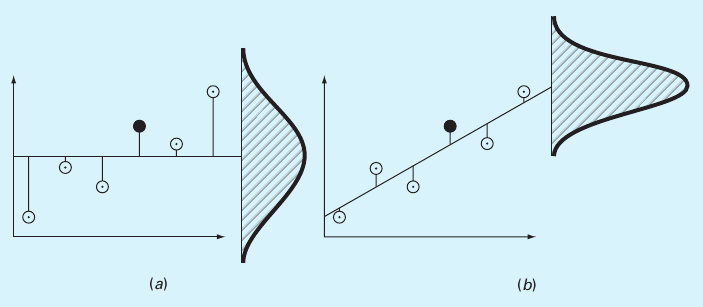
\includegraphics[width=0.5\linewidth]{fig_14_10}
	\caption{\textsf{Regression data showing (a) the spread of the data around the mean of the dependent variable and (b) the spread of the data around the best-fit line. The reduction in the spread in going from (a) to (b), as indicated by the bell-shaped curves at the right, represents the improvement due to linear regression.}}
	\label{fig:fig_14_10}
	\label{fig:fig_14_10a}
	\label{fig:fig_14_10b}
\end{figure}

\begin{figure}[H]
	\centering
	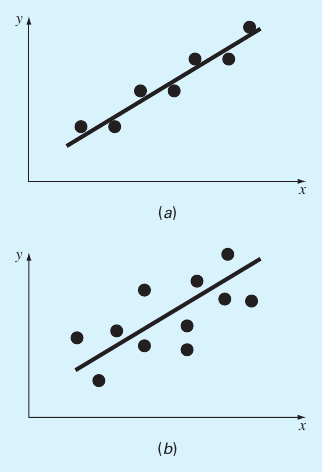
\includegraphics[width=0.5\linewidth]{fig_14_11}
	\caption{\textsf{Examples of linear regression with (a) small and (b) large residual errors.}}
	\label{fig:fig_14_11}
	\label{fig:fig_14_11a}
	\label{fig:fig_14_11b}
\end{figure}

These concepts can be used to quantify the ``goodness'' of our fit. This is particularly useful for comparison of several regressions (\ref{fig:fig_14_11a}). To do this, we return to the original data and determine the total sum of the squares around the mean for the dependent variable (in our case, $y$). As was the case for Eq. (14.18), this quantity is designated $S_t$. This is the magnitude of the residual error associated with the dependent variable prior to regression. After performing the regression, we can compute $S_r$, the sum of the squares of the residuals around the regression line with Eq. (14.17). This characterizes the residual error that remains after the regression. It is, therefore, sometimes called the unexplained sum of the squares. The difference between the two quantities, $S_t - S_r$, quantifies the improvement or error reduction due to describing the data in terms of a straight line rather than as an average value. Because the magnitude of this quantity is scale-dependent, the difference is normalized to $S_t$ to yield

\begin{equation}
	\tag{14.20}
	r^2 = \frac{S_t - S_r}{S_t}
\end{equation}

\noindent where $r^2$ is called the \textit{coefficient of determination} and $r$ is the \textit{correlation coefficient} ($=\sqrt{r^2}$). For a perfect fit, $S_r = 0$ and $r^2 = 1$, signifying that the line explains 100\% of the variability of the data. For $r^2 = 0$, $S_r = S_t$ and the fit represents no improvement. An alternative formulation for $r$ that is more convenient for computer implementation is

\begin{equation}
	\tag{14.21}
	r = \frac{n \sum (x_i y_i) - (\sum x_i) (\sum y_i)}{\sqrt{n \sum x^2_i - (\sum x_i)^2} \sqrt{n \sum y^2_i - (\sum y_i)^2}}
\end{equation}

\begin{example} Estimation of Errors for the Linear Least-Squares Fit

    \noindent\textbf{Problem Statement.}\quad Compute the total standard deviation, the standard error of the estimate, and the correlation coefficient for the fit in Example 14.4.

    \noindent\textbf{Solution.}\quad  The data can be set up in tabular form and the necessary sums computed as in Table 14.5.

    \noindent \textbf{TABLE 14.5} \quad Data and summations needed to compute the goodness-of-fit statistics
	for the data from Table 14.1.

	\begin{tabular}{lrrrrr}
		$i$ & $x_i$ & $y_i$ & $a_0 + a_1 x_i$ & $( y_i - \bar{y})^2$ & $( y_i - a_0 - a_1 x_i)^2$ \\
		1 & 10 & 25 & -39.58 & 380,535 & 4,171 \\
		2 & 20 & 70 & 155.12 & 327,041 & 7,245 \\
		3 & 30 & 380 & 349.82 & 68,579 & 911 \\
		4 & 40 & 550 & 544.52 & 8,441 & 30 \\
		5 & 50 & 610 & 739.23 & 1,016 & 16,699 \\
		6 & 60 & 1,220 & 933.93 & 334,229 & 81,837 \\
		7 & 70 & 830 & 1,128.63 & 35,391 & 89,180 \\
		8 & 80 & 1,450 & 1,323.33 & 653,066 & 16,044 \\
		$\sum$ & 360 & 5,135 & & 1,808,297 & 216,118

	\end{tabular}

    The standard deviation is [Eq. (14.3)]

	\begin{equation}
		\notag
		s_y = \frac{1,808,297}{8-1}=508.26
	\end{equation}

	\noindent and the standard error of the estimate is [Eq. (14.19)]

	\begin{equation}
		\notag
		s_{y/x} = \frac{216,118}{8-2}189.79
	\end{equation}

	\noindent Thus, because $s_{y/x} < s_y$, the linear regression model has merit. The extent of the improvement is quantified by [Eq. (14.20)]

	\begin{equation}
		\notag
		r^2 = \frac{1,808,297 - 216,118}{1,808,297} = 0.8805
	\end{equation}

	\noindent or $r = \sqrt{0.8805} = 0.9383$. These results indicate that 88.05\% of the original uncertainty has been explained by the linear model.
\end{example}

Before proceeding, a word of caution is in order. Although the coefficient of determination provides a handy measure of goodness-of-fit, you should be careful not to ascribe more meaning to it than is warranted. Just because $r^2$ is ``close'' to 1 does not mean that the fit is necessarily ``good''. For example, it is possible to obtain a relatively high value of $r^2$ when the underlying relationship between $y$ and $x$ is not even linear. Draper and Smith (1981) provide guidance and additional material regarding assessment of results for linear regression. In addition, at the minimum, you should always inspect a plot of the data along with your regression curve.

A nice example was developed by Anscombe (1973). As in Fig. 14.12, he came up with four data sets consisting of 11 data points each. Although their graphs are very different, all have the same best-fit equation, $y = 3 + 0.5 x$, and the same coefficient of determination, $r^2 = 0.67$! This example dramatically illustrates why developing plots is so valuable.

\begin{figure}[H]
	\centering
	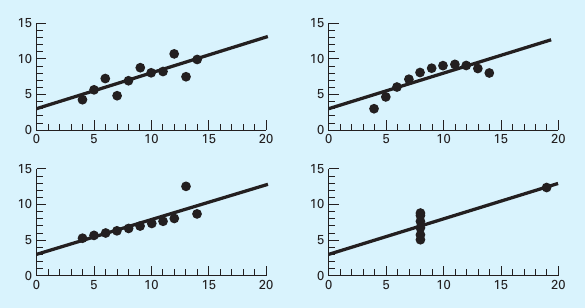
\includegraphics[width=0.5\linewidth]{fig_14_12}
	\caption{\textsf{Anscombe's four data sets along with the best-fit line, $y = 3 + 0.5x$.}}
	\label{fig:fig_14_12}
\end{figure}


\label{cha:cha_P_14_4}
\section{LINEARIZATION OF NONLINEAR RELATIONSHIPS}

Linear regression provides a powerful technique for fitting a best line to data. However, it is predicated on the fact that the relationship between the dependent and independent variables is linear. This is not always the case, and the first step in any regression analysis should be to plot and visually inspect the data to ascertain whether a linear model applies. In some cases, techniques such as polynomial regression, which is described in Chap. 15, are appropriate. For others, transformations can be used to express the data in a form that is compatible with linear regression.

One example is the \textit{exponential model}:

\begin{equation}
	\tag{14.22}
	y = a_1 e^{\beta_1 x}
\end{equation}

\noindent where $\alpha$ and $\beta_1$ are constants. This model is used in many fields of engineering and science to characterize quantities that increase (positive $\beta_1$) or decrease (negative $\beta_1$) at a rate that is directly proportional to their own magnitude. For example, population growth or radioactive decay can exhibit such behavior. As depicted in Fig. 14.13a, the equation represents a nonlinear relationship (for $\beta_1 \neq 0$) between $y$ and $x$.

Another example of a nonlinear model is the simple \textit{power equation:}

\begin{equation}
	\tag{14.23}
	y = a_2 x^{\beta_2}
\end{equation}

\noindent where $\alpha_2$ and $\beta_2$ are constant coefficients. This model has wide applicability in all fields of engineering and science. It is very frequently used to fit experimental data when the underlying model is not known. As depicted in Fig. 14.13b, the equation (for $\beta_2 \neq 0$) is nonlinear.

\begin{figure}[H]
	\centering
	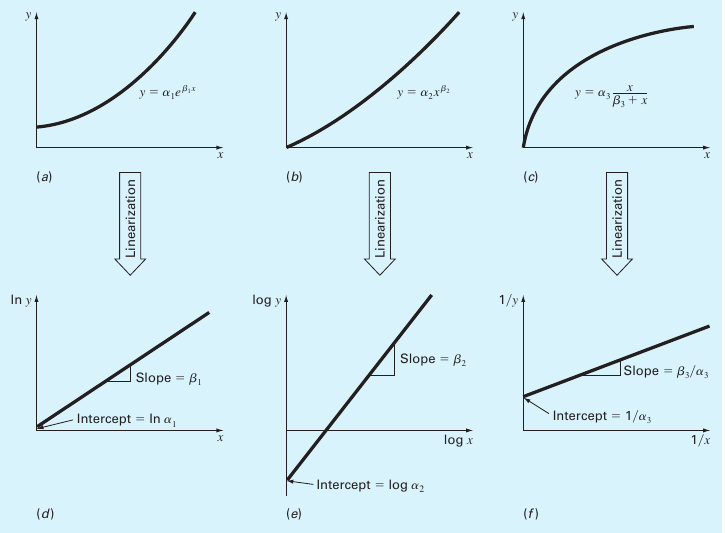
\includegraphics[width=0.5\linewidth]{fig_14_13}
	\caption{\textsf{(a) The exponential equation, (b) the power equation, and (c) the saturation-growth-rate equation. Parts (d), (e), and (f) are linearized versions of these equations that result from simple transformations.}}
	\label{fig:fig_14_13}
	\label{fig:fig_14_13a}
	\label{fig:fig_14_13b}
	\label{fig:fig_14_13c}
	\label{fig:fig_14_13d}
	\label{fig:fig_14_13e}
	\label{fig:fig_14_13f}
\end{figure}


A third example of a nonlinear model is the \textit{saturation-growth-rate equation}:

\begin{equation}
	\tag{14.24}
	y = \alpha_3 \frac{x}{\beta_3 + x}
\end{equation}

\noindent where $\alpha_3$ and $\beta_3$ are constant coefficients. This model, which is particularly well-suited for characterizing population growth rate under limiting conditions, also represents a nonlinear relationship between y and x (Fig. 14.13c) that levels off, or “saturates,” as $x$ increases. It has many applications, particularly in biologically related areas of both engineering and science.

Nonlinear regression techniques are available to fit these equations to experimental data directly. However, a simpler alternative is to use mathematical manipulations to trans form the equations into a linear form. Then linear regression can be employed to fit the equations to data.

For example, Eq. (14.22) can be linearized by taking its natural logarithm to yield

\begin{equation}
	\tag{14.25}
	\ln{y} = \ln{\alpha_1} + \beta_1 x
\end{equation}

\noindent Thus, a plot of $\ln{y}$ versus $x$ will yield a straight line with a slope of $\beta_1$ and an intercept of $\ln{\alpha_1}$ (Fig. 14.13d).

Equation (14.23) is linearized by taking its base-10 logarithm to give

\begin{equation} % Page 346
	\tag{14.26}
	\log y = \log \alpha_2 + \beta_2 \log x
\end{equation} 

\noindent Thus, a plot of log y versus log x will yield a straight line with a slope of $\beta_2$ and an intercept of $\log \alpha_2$ (Fig. 14.13e). Note that any base logarithm can be used to linearize this model. However, as done here, the base-10 logarithm is most commonly employed.

Equation (14.24) is linearized by inverting it to give

\begin{equation}
	\tag{14.27}
	\frac{1}{y} = \frac{1}{\alpha_3} + \frac{\beta_3}{\alpha_3} \frac{1}{x}
\end{equation}

\noindent Thus, a plot of $1/y$ versus $1/x$ will be linear, with a slope of $\beta_3 / \alpha_3$ and an intercept of $1 / \alpha_3$ (Fig. 14.13f).

In their transformed forms, these models can be fit with linear regression to evaluate the constant coefficients. They can then be transformed back to their original state and used for predictive purposes. The following illustrates this procedure for the power model.

\begin{example} Estimation of Errors for the Linear Least-Squares Fit

    \noindent\textbf{Problem Statement.}\quad CFit Eq. (14.23) to the data in Table 14.1 using a logarithmic transformation.

    \noindent\textbf{Solution.}\quad  The data can be set up in tabular form and the necessary sums computed as in Table 14.6.

	The means can be computed as
	
	\begin{equation}
		\notag
		\bar{x} = \frac{12.606}{8}=1.5757 \quad \bar{y} = \frac{20.515}{8} = 2.5644
	\end{equation}

	\noindent\textbf{TABLE 14.6}\quad Data and summations needed to fit the power model to the data from
	Table 14.1

	\begin{tabular}{rrrrrrr}
		$i$ & $x_i$ & $y_i$ & $\log x_i$ & $\log y_i$ & $(\log x_i )^2$ & $\log x_i \log y_i$ \\
		\hline
		1 & 10 & 25 & 1.000 & 1.398 & 1.000 & 1.398 \\
		2 & 20 & 70 & 1.301 & 1.845 & 1.693 & 2.401 \\
		3 & 30 & 380 & 1.477 & 2.580 & 2.182 & 3.811 \\
		4 & 40 & 550 & 1.602 & 2.740 & 2.567 & 4.390 \\
		5 & 50 & 610 & 1.699 & 2.785 & 2.886 & 4.732 \\
		6 & 60 & 1220 & 1.778 & 3.086 & 3.162 & 5.488 \\
		7 & 70 & 830 & 1.845 & 2.919 & 3.404 & 5.386 \\
		8 & 80 & 1450 & 1.903 & 3.161 & 3.622 & 6.016 \\
		$\sum$ &&&12.606 & 20.515 & 20.516 & 33.622

	\end{tabular}

	\begin{figure}[H]
		\centering
		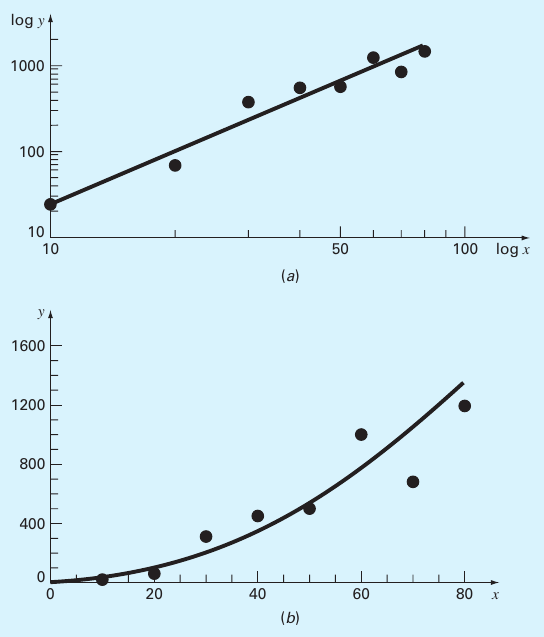
\includegraphics[width=0.5\linewidth]{fig_14_14}
		\caption{\textsf{Least-squares fit of a power model to the data from Table 14.1. (a) The fit of the transformed data.
		(b) The power equation fit along with the data.}}
		\label{fig:fig_14_14}
	\end{figure}

	\noindent The slope and the intercept can then be calculated with Eqs. (14.15) and (14.16) as

	\begin{equation}
		\notag
		a_1 = \frac{8(33.622) - 12.606(20.515)}{8(20.516) - (12.606)^2} = 1.9842
	\end{equation}

	\begin{equation}
		\notag
		a_0 = 2.5644 - 1.9842(1.5757) = -0.5620
	\end{equation}

	\noindent The least-squares fit is

	\begin{equation}
		\notag
		\log y = -0.5620 + 1.9842 \log x
	\end{equation}

	\noindent The fit, along with the data, is shown in Fig. 14.14a.

	We can also display the fit using the untransformed coordinates. To do this, the coefficients of the power model are determined as $\alpha_2 = 10^{-0.5620} = 0.2741$ and $\beta_2 = 1.9842$. Using force and velocity in place of $y$ and $x$, the least-squares fit is

	\begin{equation}
		\notag
		F = 0.2741 v ^ {1.9842}		
	\end{equation}

	\noindent This equation, along with the data, is shown in Fig. 14.14b.
\end{example}


The fits in Example 14.6 (Fig. 14.14) should be compared with the one obtained previously in Example 14.4 (Fig. 14.8) using linear regression on the untransformed data. Although both results would appear to be acceptable, the transformed result has the advantage that it does not yield negative force predictions at low velocities. Further, it is known from the discipline of fluid mechanics that the drag force on an object moving through a fluid is often well described by a model with velocity squared. Thus, knowledge from the field you are studying often has a large bearing on the choice of the appropriate model equation you use for curve fitting.


\label{cha:cha_P_14_4_1}
\subsection{General Comments on Linear Regression}

\noindent Before proceeding to curvilinear and multiple linear regression, we must emphasize the introductory nature of the foregoing material on linear regression. We have focused on the simple derivation and practical use of equations to fit data. You should be cognizant of the fact that there are theoretical aspects of regression that are of practical importance but are beyond the scope of this book. For example, some statistical assumptions that are inherent in the linear least-squares procedures are

\begin{enumerate}
	\item Each $x$ has a fixed value; it is not random and is known without error.
	\item The $y$ values are independent random variables and all have the same variance.
	\item The $y$ values for a given $x$ must be normally distributed.
\end{enumerate}

Such assumptions are relevant to the proper derivation and use of regression. For example, the first assumption means that (1) the $x$ values must be error-free and (2) the regression of $y$ versus $x$ is not the same as $x$ versus $y$. You are urged to consult other references such as Draper and Smith (1981) to appreciate aspects and nuances of regression that are beyond the scope of this book.

\label{cha:cha_P_14_5}
\section{COMPUTER APPLICATIONS}

\noindent Linear regression is so commonplace that it can be implemented on most pocket calculators. In this section, we will show how a simple M-file can be developed to determine the slope and intercept as well as to create a plot of the data and the best-fit line. We will also show how linear regression can be implemented with the built-in \texttt{polyfit} function.

\label{cha:cha_P_14_5_1}
\subsection{MATLAB M-file: \texttt{linregr}}
\noindent An algorithm for linear regression can be easily developed (Fig. 14.15). The required summations are readily computed with MATLAB's \texttt{sum} function. These are then used to compute the slope and the intercept with Eqs. (14.15) and (14.16). The routine displays the intercept and slope, the coefficient of determination, and a plot of the best-fit line along with the measurements.

A simple example of the use of this M-file would be to fit the force-velocity data analyzed in Example 14.4:

\begin{lstlisting}[numbers=none]
	>> x = [10 20 30 40 50 60 70 80];
	>> y = [25 70 380 550 610 1220 830 1450];
	>> linregr(x,y)
	r2 =
		0.8805
	ans =
		19.4702 -234.2857
\end{lstlisting}

\begin{figure}[H]
	\centering
	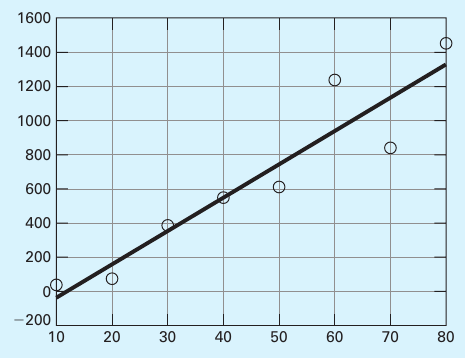
\includegraphics[width=0.5\linewidth]{fig_14_5_1_u_1}
\end{figure}

It can just as easily be used to fit the power model (Example 14.6) by applying the
\texttt{log10} function to the data as in

\begin{lstlisting}[numbers=none]
	>> linregr(log10(x),log10(y))
	r2 =
		0.9481
	ans =
		1.9842	-0.5620
\end{lstlisting}

\begin{figure}[H]
	\centering
	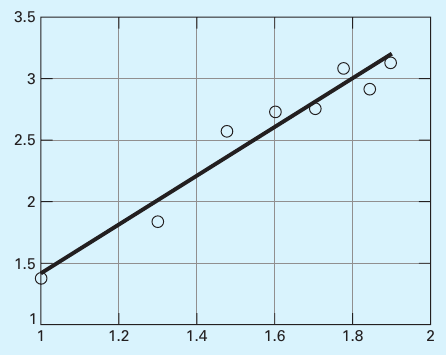
\includegraphics[width=0.5\linewidth]{fig_14_5_1_u_2}
\end{figure}

\begin{figure}[H]
	\centering
	\begin{lstlisting}[numbers=none]
		function [a, r2] = linregr(x,y)
		% linregr: linear regression curve fitting
		%	[a, r2] = linregr(x,y): Least squares fit of straight
		%		line to data by solving the normal equations

		% input:
		%	x = independent variable
		%	y = dependent variable
		% output:
		%	a = vector of slope, a(1), and intercept, a(2)
		%	r2 = coefficient of determination

		n = length(x);
		if length(y)~=n, error('x and y must be same length'); end
		x = x(:); y = y(:);
		% convert to column vectors
		sx = sum(x); sy = sum(y);
		sx2 = sum(x.*x); sxy = sum(x.*y); sy2 = sum(y.*y);
		a(1) = (n*sxy-sx*sy)/(n*sx2-sx^2);
		a(2) = sy/n-a(1)*sx/n;
		r2 = ((n*sxy-sx*sy)/sqrt(n*sx2-sx^2)/sqrt(n*sy2-sy^2))^2;
		% create plot of data and best fit line
		xp = linspace(min(x),max(x),2);
		yp = a(1)*xp+a(2);
		plot(x,y,'o',xp,yp)
		grid on
	\end{lstlisting}
	\caption{\textsf{An M-file to implement linear regression.}}
	\label{fig:fig_14_15}
\end{figure}

\label{cha:cha_P_14_5_2} %351
\subsection{MATLAB Functions: \texttt{polyfit} and \texttt{polyval}}

\noindent MATLAB has a built-in function \texttt{polyfit} that fits a least-squares \textit{n}th-order polynomial to data. It can be applied as in

\begin{lstlisting}[numbers=none]
>> p = polyfit(x, y, n)
\end{lstlisting}

\noindent where $x$ and $y$ are the vectors of the independent and the dependent variables, respectively, and $n =$ the order of the polynomial. The function returns a vector $p$ containing the polynomial's coefficients. We should note that it represents the polynomial using decreasing powers of $x$ as in the following representation:

\begin{equation}
	\notag
	f(x) = p_1x^n + p_2x^{n-1} + \cdots + p_n x + p_{n + 1}
\end{equation}

Because a straight line is a first-order polynomial, \verb|polyfit(x,y,1)| will return the slope and the intercept of the best-fit straight line.

\begin{lstlisting}[numbers=none]
>> x = [10 20 30 40 50 60 70 80];
>> y = [25 70 380 550 610 1220 830 1450];
>> a = polyfit(x,y,1)
a =
	19.4702 -234.2857
\end{lstlisting}

\noindent Thus, the slope is 19.4702 and the intercept is -234.2857.

Another function, \texttt{polyval}, can then be used to compute a value using the coefficients. It has the general format:

\begin{lstlisting}[numbers=none]
>> y = polyval(p, x)
\end{lstlisting}

\noindent where $p =$ the polynomial coefficients, and $y =$ the best-fit value at $x$. For example,

\begin{lstlisting}[numbers=none]
>> y = polyval(a,45)
y =
	641.8750
\end{lstlisting}

\bigskip

% ENZYME KINETICS
\textbf{Background.} \textit{Enzymes} act as catalysts to speed up the rate of chemical reactions in living cells. In most cases, they convert one chemical, the \textit{substrate},into another, the \textit{product}. The \textit{Michaelis-Menten} equation is commonly used to describe such reactions:

\begin{equation}
	\tag{14.28}
	v = \frac{v_m[S]}{k_s + [S]}
\end{equation}

\noindent where $v =$ the initial reaction velocity, $v_m =$ the maximum initial reaction velocity, $[S] =$ substrate concentration, and $k_s =$ a half-saturation constant. As in Fig. 14.16, the equation describes a saturating relationship which levels off with increasing $[S]$. The graph also illustrates that the \textit{half-saturation constant} corresponds to the substrate concentration at which the velocity is half the maximum.

\begin{figure}[H] % Page 352
	\centering
	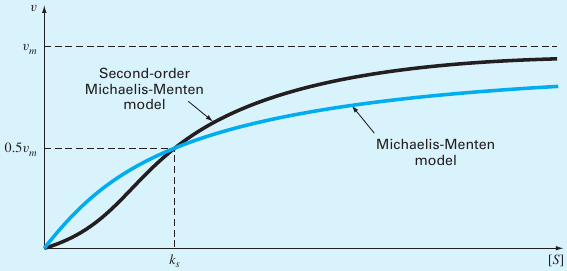
\includegraphics[width=0.5\linewidth]{fig_14_16}
	\caption{\textsf{Two versions of the Michaelis-Menten model of enzyme kinetics.}}
	\label{fig:fig_14_16}
\end{figure}

Although the Michaelis-Menten model provides a nice starting point, it has been refined and extended to incorporate additional features of enzyme kinetics. One simple extension involves so-called \textit{allosteric enzymes}, where the binding of a substrate molecule at one site leads to enhanced binding of subsequent molecules at other sites. For cases with two interacting bonding sites, the following second-order version often results in a better fit:

\begin{equation}
	\tag{14.29}
	v = \frac{v_m {[S]}^2}{k^2_s + {[S]}^2}
\end{equation}

\noindent This model also describes a saturating curve but, as depicted in Fig. 14.16, the squared concentrations tend to make the shape more \textit{sigmoid},or S-shaped.

Suppose that you are provided with the following data:

\begin{tabular}{l c c c c c c c c c}
	[S] &1.3 & 1.8 & 3  &  4.5  & 6  &   8   & 9 \\
	v  & 0.07 &0.13 &0.22 &0.275& 0.335& 0.35 &0.36
\end{tabular}

\noindent Employ linear regression to fit these data with linearized versions of Eqs. (14.28) and (14.29). Aside from estimating the model parameters, assess the validity of the fits with both statistical measures and graphs.

\textbf{Solution.} Equation (14.28), which is in the format of the saturation-growth-rate model (Eq. 14.24), can be linearized by inverting it to give (recall Eq. 14.27)

\begin{equation}
	\notag
	\frac{1}{v} = \frac{1}{v_m} + \frac{k_s}{v_m} \frac{1}{[S]}
\end{equation}

\noindent The \texttt{linregr} function from Fig. 14.15 can then be used to determine the least-squares fit:

\begin{lstlisting}[numbers=none] 
>> S=[1.3 1.8 3 4.5 6 8 9];
>> v=[0.07 0.13 0.22 0.275 0.335 0.35 0.36];
>> [a,r2]=linregr(1./S,1./v)
a =
16.4022
 0.1902
r2 =
0.9344
\end{lstlisting}

\noindent The model coefficients can then be calculated as

\begin{lstlisting}[numbers=none] 
>> vm=1/a(2)
vm =
5.2570
>> ks=vm*a(1)
ks =
86.2260
\end{lstlisting}

\noindent Thus, the best-fit model is

\begin{equation}
	\notag
	v = \frac{5.2570[S]}{86.2260 + [S]}
\end{equation}

Although the high value of $r^2$ might lead you to believe that this result is acceptable, inspection of the coefficients might raise doubts. For example, the maximum velocity (5.2570) is much greater than the highest observed velocity (0.36). In addition, the half-saturation rate (86.2260) is much bigger than the maximum substrate concentration (9).

The problem is underscored when the fit is plotted along with the data. Figure 14.17a shows the transformed version. Although the straight line follows the upward trend, the data clearly appear to be curved. When the original equation is plotted along with the data in the untransformed version (Fig. 14.17b), the fit is obviously unacceptable. The data are clearly leveling off at about 0.36 or 0.37. If this is correct, an eyeball estimate would suggest that $v_m$ should be about 0.36, and $k_s$ should be in the range of 2 to 3.

Beyond the visual evidence, the poorness of the fit is also reflected by statistics like the coefficient of determination. For the untransformed case, a much less acceptable result of $r^2 = 0.6406$ is obtained.


The foregoing analysis can be repeated for the second-order model. Equation (14.28) can also be linearized by inverting it to give

\begin{equation}
	\notag
	\frac{1}{v} = \frac{1}{v_m} + \frac{k^2_s}{v_m} \frac{1}{[S]^2}
\end{equation}

The \texttt{linregr} function from Fig. 14.15 can again be used to determine the least-squares fit:

\begin{lstlisting}[numbers=none] 
>> [a,r2]=linregr(1./S.^2,1./v)
a =
19.3760
 2.4492
r2 =
0.9929
\end{lstlisting}

% Page 354
\begin{figure}[H] 
	\centering
	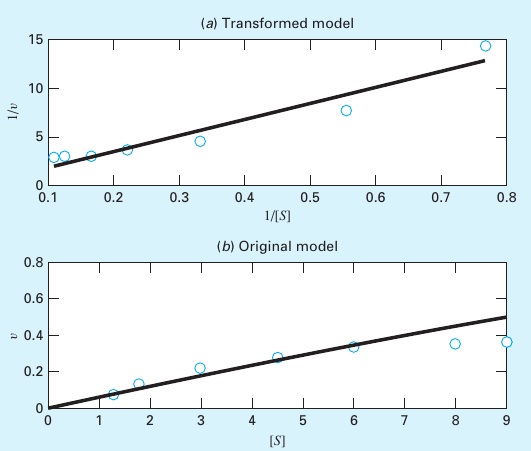
\includegraphics[width=0.5\linewidth]{fig_14_17}
	\caption{\textsf{Plots of least-squares fit (line) of the Michaelis-Menten model along with data (points). The plot in (a) shows the transformed fit, and (b) shows how the fit looks when viewed in the untransformed, original form.}}
	\label{fig:fig_14_17}
\end{figure}

\noindent The model coefficients can then be calculated as

\begin{lstlisting}[numbers=none] 
>> vm=1/a(2)
vm =
0.4083
>> ks=sqrt(vm*a(1))
ks =
2.8127
\end{lstlisting}

\noindent Substituting these values into Eq. (14.29) gives

\begin{equation}
	\notag
	v = \frac{0.4083[S]^2}{7.911 + [S]^2}
\end{equation}

Although we know that a high $r^2$ does not guarantee of a good fit, the fact that it is very high (0.9929) is promising. In addition, the parameters values also seem consistent with the trends in the data; that is, the $k_m$ is slightly greater than the highest observed velocity and the half-saturation rate is lower than the maximum substrate concentration (9).

\begin{figure}[H] 
	\centering
	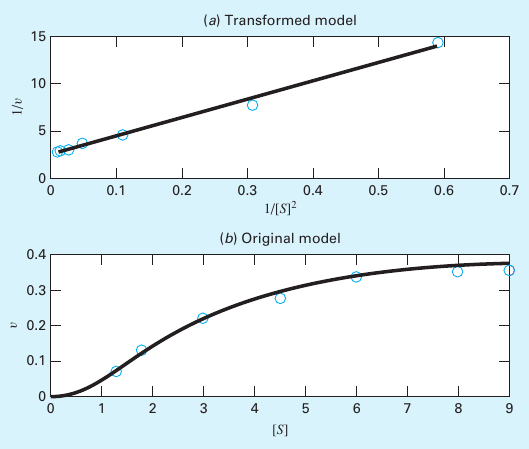
\includegraphics[width=0.5\linewidth]{fig_14_18}
	\caption{\textsf{Plots of least-squares fit (line) of the second-order Michaelis-Menten model along with data (points). The plot in (a) shows the transformed fit, and (b) shows the untransformed, original form.}}
	\label{fig:fig_14_18}
\end{figure}

The adequacy of the fit can be assessed graphically. As in Fig. 14.18a, the transformed results appear linear. When the original equation is plotted along with the data in the untransformed version (Fig. 14.18b), the fit nicely follows the trend in the measurements. Beyond the graphs, the goodness of the fit is also reflected by the fact that the coefficient of determination for the untransformed case can be computed as $r^2 = 0.9896$.

Based on our analysis, we can conclude that the second-order model provides a good fit of this data set. This might suggest that we are dealing with an allosteric enzyme. 

Beyond this specific result, there are a few other general conclusions that can be drawn from this case study. First, we should never solely rely on statistics such as $r^2$ as the sole basis of assessing goodness of fit. Second, regression equations should always be assessed graphically. And for cases where transformations are employed, a graph of the untransformed model and data should always be inspected. 

Finally, although transformations may yield a decent fit of the transformed data, this does not always translate into an acceptable fit in the original format. The reason that this might occur is that minimizing squared residuals of transformed data is not the same as for the untransformed data. Linear regression assumes that the scatter of points around the best-fit line follows a Gaussian distribution,  and that the standard deviation is the same at every value of the dependent variable. These assumptions are rarely true after transforming data. 

As a consequence of the last conclusion, some analysts suggest that rather than using linear transformations, nonlinear regression should be employed to fit curvilinear data. In this approach, a best-fit curve is developed that directly minimizes the untransformed residuals. We will describe how this is done in Chap. 15.

\setlength{\tabcolsep}{3pt}

\bigskip
\noindent\textbf{PROBLEMS}\\

\begin{multicols}{2}
    \noindent\textbf{14.1} Given the data

	\noindent \begin{tabular}{ c c c c c }
		0.90 & 1.42 & 1.30 & 1.55 & 1.63 \\
		1.32 & 1.35 & 1.47 & 1.95 & 1.66 \\
		1.96 & 1.47 & 1.92 & 1.35 & 1.05 \\
		1.85 & 1.74 & 1.65 & 1.78 & 1.71 \\
		2.29 & 1.82 & 2.06 & 2.14 & 1.27
	\end{tabular}

	\noindent Determine \textbf{(a)} the mean, \textbf{(b)} median, \textbf{(c)} mode, \textbf{(d)} range,
	\textbf{(e)} standard deviation, \textbf{(f)} variance, and \textbf{(g)} coefficient of
	variation.	


	\noindent\textbf{14.2}  Construct a histogram from the data from Prob. 14.1. Use a range from 0.8 to 2.4 with intervals of 0.2.

	\noindent\textbf{14.3} Given the data

	\noindent \begin{tabular}{c c c c c c c}
		29.65 & 28.55 & 28.65 & 30.15 & 29.35 & 29.75 & 29.25 \\
		30.65 & 28.15 & 29.85 & 29.05 & 30.25 & 30.85 & 28.75 \\
		29.65 & 30.45 & 29.15 & 30.45 & 33.65 & 29.35 & 29.75 \\
		31.25 & 29.45 & 30.15 & 29.65 & 30.55 & 29.65 & 29.25
	\end{tabular}

	\noindent Determine \textbf{(a)} the mean, \textbf{(b)} median, \textbf{(c)} mode, \textbf{(d)} range,
	\textbf{(e)} standard deviation, \textbf{(f)} variance, and \textbf{(g)} coefficient of
	variation.
	\textbf{(h)} Construct a histogram. Use a range from 28 to 34 with
	increments of 0.4.
	\textbf{(i)} Assuming that the distribution is normal, and that your
	estimate of the standard deviation is valid, compute the
	range (i.e., the lower and the upper values) that encompasses 68\% of the readings. Determine whether this is a
	valid estimate for the data in this problem.

	\noindent\textbf{14.4} Using the same approach as was employed to derive
	Eqs. (14.15) and (14.16), derive the least-squares fit of the
	following model:

	$$y = a_1 x + e$$

	\noindent That is, determine the slope that results in the least-squares fit for a straight line with a zero intercept. Fit the following data with this model and display the result graphically.

	\noindent \begin{tabular}{c c c c c c c c c c }
	 	\textbf{x} & 2 & 4 & 6 & 7 & 10 & 11 & 		14 & 		17 & 		20 \\
	  	\textbf{y} & 4 & 5 & 6 & 5 & 8 & 8 & 6 & 9 & 		12
	\end{tabular}

	\noindent\textbf{14.5} Use least-squares regression to fit a straight line to

	\noindent \begin{tabular}{c c c c c c c c c c c  }
 		x & 0 & 2 & 4 & 6 & 9 & 11 & 12 & 15 & 17 & 19 \\
 		y & 5 & 6 & 7 & 6 & 9 & 8 & 8 & 10 & 12 & 12
   	\end{tabular}

   	\noindent Along with the slope and intercept, compute the standard
	   error of the estimate and the correlation coefficient. Plot the
	   data and the regression line. Then repeat the problem, but
	   regress $x$ versus $y$ - that is, switch the variables. Interpret
	   your results.

	\noindent\textbf{14.6} Fit a power model to the data from Table 14.1, but use
	natural logarithms to perform the transformations.

	\noindent\textbf{14.7} The following data were gathered to determine the
	relationship between pressure and temperature of a fixed
	volume of 1 kg of nitrogen. The volume is 10 m$^3$.

	\noindent \begin{tabular}{l c c c c c c c c c c  }
		\textbf{T, $^\circ$C} & -40 & 0 & 40 & 80 & 120 & 160 \\
		\textbf{p, N/m$^2$} & 6900 & 8100 & 9350 & 10,500 & 11,700 & 12,800
  	\end{tabular}

	\noindent Employ the ideal gas law $pV = nRT$ to determine $R$ on the
	basis of these data. Note that for the law, $T$ must be expressed
	in kelvins.

	\noindent\textbf{14.8} Beyond the examples in Fig. 14.13, there are other
	models that can be linearized using transformations. For
	example,

	$$y = a_4 x e^{\beta_4 x}$$

	\noindent Linearize this model and use it to estimate $\alpha_4$ and $\beta_4$ based
	on the following data. Develop a plot of your fit along with
	the data.

	\noindent \begin{tabular}{c c c c c c c c c c}
		\textbf{x} & 0.1 & 0.2 & 0.4 & 0.6 & 0.9 & 1.3 & 1.5 & 1.7 & 1.8 \\
		\textbf{y} & 0.75 & 1.25 & 1.45 & 1.25 & 0.85 & 0.55 & 0.35 & 0.28 & 0.18	
  	\end{tabular}

	\noindent\textbf{14.9} The concentration of \textit{E. coli} bacteria in a swimming
	area is monitored after a storm:

	\noindent \begin{tabular}{l c c c c c c}
		\textbf{t (hr)} & 4 & 8 & 12 & 16 & 20 & 24 \\
		\textbf{c (CFU/100 mL)} & 1600 & 1320 & 1000 & 890 & 650 & 560
  	\end{tabular}

	\noindent The time is measured in hours following the end of the storm
	and the unit CFU is a ``colony forming unit.'' Use this data to
	estimate \textbf{(a)} the concentration at the end of the storm ($t = 0$)
	and \textbf{(b)} the time at which the concentration will reach
	200 CFU/100 mL. Note that your choice of model should
	be consistent with the fact that negative concentrations are
	impossible and that the bacteria concentration always decreases with time.

	\noindent\textbf{14.10} Rather than using the base-$e$ exponential model
	(Eq. 14.22), a common alternative is to employ a base-10
	model:

	$$y = \alpha_5 10^{\beta_5 x}$$

	\noindent When used for curve fitting, this equation yields identical
	results to the base-$e$ version, but the value of the exponent
	parameter ($\beta_5$) will differ from that estimated with Eq.14.22
	($\beta_1$). Use the base-10 version to solve Prob. 14.9. In addition, develop a formulation to relate $\beta_1$ to $\beta_5$ .

	\noindent\textbf{14.11} Determine an equation to predict metabolism rate as a
	function of mass based on the following data. Use it to predict the metabolism rate of a 200-kg tiger.

	\noindent \begin{tabular}{l c c }
		\textbf{Animal} & \textbf{Mass (kg)} & \textbf{Metabolism (watts)} \\
		\hline
		Cow &  400 &  270 \\
		Human &  70 &  82 \\ 
		Sheep &  45 &  50 \\ 
		Hen &  2 &  4.8 \\ 
		Rat &  0.3 &  1.45 \\ 
		Dove &  0.16 &  0.97
  	\end{tabular}

	\noindent\textbf{14.12} On average, the surface area $A$ of human beings is
	related to weight $W$ and height $H$. Measurements on a number of individuals of height 180 cm and different weights
	(kg) give values of $A$ (m$^2$) in the following table:

	\noindent \begin{tabular}{l c c c c c c c c c}
		\textbf{W (kg)} & 70 & 75 & 77 & 80 & 82 & 84 & 87 & 90 \\
		\textbf{A (m2)} & 2.10 & 2.12 & 2.15 & 2.20 & 2.22 & 2.23 & 2.26 & 2.30 &
  	\end{tabular}

	\noindent Show that a power law $A = aW^b$ fits these data reasonably
	well. Evaluate the constants $a$ and $b$, and predict what the
	surface area is for a 95-kg person.

	\noindent\textbf{14.13} Fit an exponential model to

	\noindent \begin{tabular}{l c c c c c c }
		\textbf{x} & 0.4 & 0.8 & 1.2 & 1.6 & 2 & 2.3 \\
		\textbf{y} & 800 & 985 & 1490 & 1950 & 2850 & 3600
  	\end{tabular}

	\noindent Plot the data and the equation on both standard and semi-logarithmic graphs with the MATLAB \texttt{subplot} function.

	\noindent\textbf{14.14} An investigator has reported the data tabulated below
	for an experiment to determine the growth rate of bacteria
	$k$ (per d) as a function of oxygen concentration $c$ (mg/L). It
	is known that such data can be modeled by the following
	equation:

	$$k = \frac{k_{\text{max}} c^2}{c_s + c^2}$$

	\noindent where $c_s$ and $k_{\text{max}}$ are parameters. Use a transformation to
	linearize this equation. Then use linear regression to estimate $c_s$ and $k_{\text{max}}$ and predict the growth rate at $c$ = 2 mg/L.

	\noindent \begin{tabular}{l c c c c c}
		\textbf{c} & 0.5 & 0.8 & 1.5 & 2.5 \\
		\textbf{k} & 1.1 & 2.5 & 5.3 & 7.6 & 8.9
  	\end{tabular}

	\noindent\textbf{14.15} Develop an M-file function to compute descriptive
	statistics for a vector of values. Have the function determine
	and display number of values, mean, median, mode, range,
	standard deviation, variance, and coefficient of variation. In
	addition, have it generate a histogram. Test it with the data
	from Prob. 14.3.

	\noindent\textbf{14.16}  Modify the \texttt{linregr} function in Fig. 14.15 so that it
	\textbf{(a)} computes and returns the standard error of the estimate,
	and \textbf{(b)} uses the \texttt{subplot} function to also display a plot of
	the residuals (the predicted minus the measured $y$) versus $x$.

	\noindent\textbf{14.17} Develop an M-file function to fit a power model.
	Have the function return the best-fit coefficient $\alpha_2$ and
	power $\beta_2$ along with the $r^2$ for the untransformed model. In
	addition, use the \texttt{subplot} function to display graphs of both
	the transformed and untransformed equations along with the
	data. Test it with the data from Prob. 14.11.

	\noindent\textbf{14.18} The following data show the relationship between the
	viscosity of SAE 70 oil and temperature. After taking the log
	of the data, use linear regression to find the equation of the
	line that best fits the data and the $r^2$ value.

	\noindent \begin{tabular}{l c c c c}
		\textbf{Temperature, $^\circ$C} & 26.67 & 93.33 & 148.89 & 315.56 \\
		\textbf{Viscosity, $\mu$, N $\cdot$ s/m$^2$} & 1.35 & 0.085 & 0.012 & 0.00075
  	\end{tabular}

	\noindent\textbf{14.19} You perform experiments and determine the following values of heat capacity $c$ at various temperatures $T$ for a gas:

	\noindent \begin{tabular}{l c c c c c c}
		\textbf{T} & -50 & -30 & 0 & 60 & 90 & 110 \\
		\textbf{c} & 1250 & 1280 & 1350 & 1480 & 1580 & 1700
  	\end{tabular}

	\noindent Use regression to determine a model to predict $c$ as a function of $T$.

	\noindent\textbf{14.20} It is known that the tensile strength of a plastic increases as a function of the time it is heat treated. The following data are collected:

	\noindent \begin{tabular}{l c c c c c c c c c c}
		\textbf{Time} & 10 & 15 & 20 & 25 & 40 & 50 & 55 & 60 & 75 \\
		\textbf{Tensile Strength} & 5 & 20 & 18 & 40 & 33 & 54 & 70 & 60 & 78
  	\end{tabular}

	\noindent \textbf{(a)} Fit a straight line to these data and use the equation to
	determine the tensile strength at a time of 32 min.


	\noindent \textbf{(b)} Repeat the analysis but for a straight line with a zero
	intercept.

	\noindent\textbf{14.21}  The following data were taken from a stirred tank reactor for the reaction $A \rightarrow B$. Use the data to determine the
	best possible estimates for $k_{01}$ and $E_1$ for the following
	kinetic model:

	$$- \frac{d A}{d t} = k _{01} e^{-E_1 / RT} A$$

	\noindent where $R$ is the gas constant and equals 0.00198 kcal/mol/K.

	\noindent \begin{tabular}{l c c c c c c c c}
		\textbf{-dA/dt (moles/L/s)} & 460 & 960 & 2485 & 1600 & 1245 \\ 
		\textbf{A (moles/L)} & 200 & 150 & 50 & 20 & 10 \\
		\textbf{T (K)} & 280 & 320 & 450 & 500 & 550
	\end{tabular}

	\noindent\textbf{14.22} Concentration data were collected at 15 time points
	for the polymerization reaction:

	$$x A + y B \rightarrow A_x B_y$$

	\noindent We assume the reaction occurs via a complex mechanism
	consisting of many steps. Several models have been hypothesized, and the sum of the squares of the residuals had been
	calculated for the fits of the models of the data. The results are shown below. Which model best describes the data (statistically)? Explain your choice.


	\noindent \begin{tabular}{l c c c}
		 & \textbf{Model A} & \textbf{Model B} & \textbf{Model C} \\
		\hline
		\textbf{S$_r$} & 135 & 105 & 100 \\
		\textbf{Number of Model} \\
		\textbf{Parameters Fit} & 2 & 3 & 5
  	\end{tabular}

	\noindent\textbf{14.23} Below are data taken from a batch reactor of bacterial
	growth (after lag phase was over). The bacteria are allowed
	to grow as fast as possible for the first 2.5 hours, and then
	they are induced to produce a recombinant protein, the production of which slows the bacterial growth significantly.
	The theoretical growth of bacteria can be described by

	$$\frac{d X}{dt} = \mu X$$

	\noindent where $X$ is the number of bacteria, and $\mu$ is the specific
	growth rate of the bacteria during exponential growth. Based
	on the data, estimate the specific growth rate of the bacteria
	during the first 2 hours of growth and during the next 4 hours
	of growth.

	\noindent \begin{tabular}{l c c c c c c c c}
		\textbf{Time,} \\
		\textbf{h} &  0 &  1 &  2 &  3 &  4 &  5 &  6 \\
		\textbf{[Cells],} \\
		\textbf{g/L} & 0.100 & 0.335 & 1.102 & 1.655 & 2.453 & 3.702 & 5.460
	\end{tabular}

	\noindent\textbf{14.24} A transportation engineering study was conducted to
	determine the proper design of bike lanes. Data were gathered on bike-lane widths and average distance between bikes
	and passing cars. The data from 9 streets are

	\noindent \begin{tabular}{l c c c c c c c c c c c c}
		\textbf{Distance, m} & 2.4 & 1.5 & 2.4 & 1.8 & 1.8 & 2.9 & 1.2 & 3 & 1.2 \\
		\textbf{Lane Width, m} & 2.9 & 2.1 & 2.3 & 2.1 & 1.8 & 2.7 & 1.5 & 2.9 & 1.5
	\end{tabular}

	\noindent \textbf{(a)} Plot the data.

	\noindent \textbf{(b)} Fit a straight line to the data with linear regression. Add this line to the plot.

	\noindent \textbf{(c)} If the minimum safe average distance between bikes and passing cars is considered to be 1.8 m, determine the corresponding minimum lane width.

	\noindent\textbf{14.25}  In water-resources engineering, the sizing of reservoirs depends on accurate estimates of water flow in the
	river that is being impounded. For some rivers, long-term
	historical records of such flow data are difficult to obtain. In
	contrast, meteorological data on precipitation are often
	available for many years past. Therefore, it is often useful to determine a relationship between flow and precipitation.
	This relationship can then be used to estimate flows for
	years when only precipitation measurements were made.
	The following data are available for a river that is to be
	dammed:

	\noindent \begin{tabular}{l c c c c c c c c c c}
		\textbf{Precip.,} \\
		\textbf{cm/yr} & 88.9 & 108.5 & 104.1 & 139.7 & 127 & 94 & 116.8 & 99.1 \\
		\textbf{Flow,} \\
		\textbf{m$^3$/s} & 14.6 & 16.7 & 15.3 & 23.2 & 19.5 & 16.1 & 18.1 & 16.6
	\end{tabular}	

		\noindent \textbf{(a)} Plot the data.

	\noindent \textbf{(b)} Fit a straight line to the data with linear regression.
Superimpose this line on your plot.

	\noindent \textbf{(c)} Use the best-fit line to predict the annual water flow if
the precipitation is 120 cm.

	\noindent \textbf{(d)} If the drainage area is 1100 km$^2$, estimate what fraction
of the precipitation is lost via processes such as evaporation, deep groundwater infiltration, and consumptive
use.

	\noindent\textbf{14.26}  The mast of a sailboat has a cross-sectional area of
	10.65 cm$^2$ and is constructed of an experimental aluminum
	alloy. Tests were performed to define the relationship between stress and strain. The test results are

	\noindent \begin{tabular}{l c c c c c c c c c c}
		\textbf{Strain,} \\
		\textbf{cm/cm} & 0.0032 & 0.0045 & 0.0055 & 0.0016 & 0.0085 & 0.0005 \\
		\textbf{Stress,} \\
		\textbf{N/cm$^2$} & 4970 & 5170 & 5500 & 3590 & 6900 & 1240
	\end{tabular}

	\noindent The stress caused by wind can be computed as $F/A_c$ where $F$ = force in the mast and $A_c$ = mast's cross-sectional area. This value can then be substituted into Hooke's law to determine the mast's deflection, $\Delta L$ = strain $\times L$, where $L$ = the mast's length. If the wind force is 25,000 N, use the data to estimate the deflection of a 9-m mast.

	\noindent\textbf{14.27} The following data were taken from an experiment
	that measured the current in a wire for various imposed voltages:

	\noindent \begin{tabular}{l c c c c c c c c c c}
		\textbf{$V$, V} & 2 & 3 & 4 & 5 & 7 & 10 \\
		\textbf{$i$, A} & 5.2 & 7.8 & 10.7 & 13 & 19.3 & 27.5
	\end{tabular}

	\noindent \textbf{(a)} On the basis of a linear regression of this data, determine
current for a voltage of 3.5 V. Plot the line and the data
and evaluate the fit.

\noindent \textbf{(b)} Redo the regression and force the intercept to be zero.

	\noindent\textbf{14.28} An experiment is performed to determine the \% elongation of electrical conducting material as a function of temperature. The resulting data are listed below. Predict the \%
	elongation for a temperature of 400 $^\circ$C.

	\noindent \begin{tabular}{l c c c c c c c c c c}
		\textbf{Temperature, $^\circ$C} & 200 & 250 & 300 & 375 & 425 & 475 & 600 \\
		\textbf{\% Elongation} & 7.5 & 8.6 & 8.7 & 10 & 11.3 & 12.7 & 15.3
	\end{tabular}

	\noindent\textbf{14.29} The population $p$ of a small community on the outskirts of a city grows rapidly over a 20-year period:

	\noindent \begin{tabular}{l c c c c c c c c c c}
		\textbf{t} & 0 & 5 & 10 & 15 & 20 \\
		\textbf{p} & 100 & 200 & 450 & 950 & 2000
	\end{tabular}

	\noindent As an engineer working for a utility company, you must
	forecast the population 5 years into the future in order to anticipate the demand for power. Employ an exponential
	model and linear regression to make this prediction.

	\noindent\textbf{14.30} The velocity u of air flowing past a flat surface is
	measured at several distances y away from the surface. Fit a
	curve to this data assuming that the velocity is zero at the
	surface ($y = 0$). Use your result to determine the shear stress
	($du/dy$) at the surface.

	\noindent \begin{tabular}{l c c c c c c c c c c}
		\textbf{$y$, m} & 0.002 & 0.006 & 0.012 & 0.018 & 0.024 \\
		\textbf{$u$, m/s} & 0.287 & 0.899 & 1.915 & 3.048 & 4.299
	\end{tabular}

	\noindent\textbf{14.31} \textit{Andrade's equation} has been proposed as a model of the effect of temperature on viscosity:

	$$ \mu = De^{B/T_a}$$

	\noindent where $\mu$ = dynamic viscosity of water ($10^{-3}$ N$\cdot$s/m$^2$), $T_a$ = absolute temperature (K), and $D$ and $B$ are parameters. Fit this model to the following data for water:

	\noindent \begin{tabular}{l c c c c c c c c c c}
		\textbf{T} & 0 & 5 & 10 & 20 & 30 & 40 \\
		\textbf{$\mu$} & 1.787 & 1.519 & 1.307 & 1.002 & 0.7975 & 0.6529
	\end{tabular}

	\noindent\textbf{14.32} Perform the same computation as in Example 14.2,
	but in addition to the drag coefficient, also vary the mass
	uniformly by $\pm 10\%$.

	\noindent\textbf{14.33} Perform the same computation as in Example 14.3,
	but in addition to the drag coefficient, also vary the mass
	normally around its mean value with a coefficient of variation of 5.7887\%.

	\noindent\textbf{14.34}  Manning's formula for a rectangular channel can be
	written as

	$$Q = \frac{1}{n_m} \frac{(BH) ^ {5/3}}{(B+2H) ^ {2/3}} \sqrt{S}$$

	\noindent where $Q$ = flow (m$^3$/s), $n_m$ = a roughness coefficient, $B$ =
	width (m), $H$ = depth (m), and $S$ = slope. You are applying
	this formula to a stream where you know that the width = 20 m
	and the depth = 0.3 m. Unfortunately, you know the roughness and the slope to only a $\pm 10\%$ precision. That is, you
	know that the roughness is about 0.03 with a range from 0.027
	to 0.033 and the slope is 0.0003 with a range from 0.00027
	to 0.00033. Assuming uniform distributions, use a Monte
	Carlo analysis with $n$ = 10,000 to estimate the distribution
	of flow.

	\noindent\textbf{14.35} A Monte Carlo analysis can be used for optimization.
	For example, the trajectory of a ball can be computed with

	\begin{equation}
		\tag{P14.35}
		y = (\tan \theta_0)x - \frac{g}{2 v^2_0 \cos ^2 \theta_0} x^2 + y_0
	\end{equation}

	\noindent where $y$ = the height (m), $\theta_0$ = the initial angle (radians),
	$v_0$ = the initial velocity (m/s), $g$ = the gravitational constant =
	9.81 m/s$^2$, and $y_0$ = the initial height (m). Given $y_0$ = 1 m,
	$v_0$ = 25 m/s, and $\theta_0 = 50$ $^\circ$C, determine the maximum height
	and the corresponding $x$ distance (\textbf{a}) analytically with calculus and (\textbf{b}) numerically with Monte Carlo simulation. For
	the latter, develop a script that generates a vector of 10,000
	uniformly-distributed values of $x$ between 0 and 60 m. Use
	this vector and Eq. P14.35 to generate a vector of heights.
	Then, employ the \texttt{max} function to determine the maximum
	height and the associated $x$ distance.
\end{multicols}

\end{document}
